\section{Applications}

\begin{figure}[!ht]
\begin{center}
        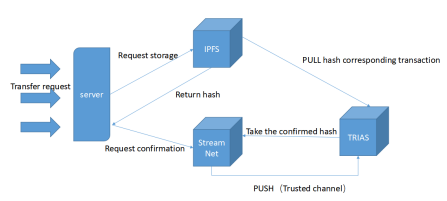
\includegraphics[width=0.50\textwidth]{figures/trias.png}
        \caption{StreamNet shows the TRIAS transfer request cache}
        \label{trias}
\end{center}
\end{figure}

\subsection{Using StreamNet in conjunction with IPFS to cache TRIAS transfer requests}
StreamNet can be used to cache and pre-confirm other low-traffic blockchain systems because of its high throughput. 
$TRIAS$ as a cross-blockchain system can take advantage of this feature to achieve ability of elasticity.
The structure is shown in Figure~\ref{trias}. 
There is a distributed transaction service. 
When an transaction request comes over, it first stores the information in the $IPFS$ and gets a hash.
Then constructs node in StreamNet using this hash.
When the traffic is small, StreamNet can directly push the hash of the transaction to $TRIAS$ after confirming it, 
so $TRIAS$ can get the specific transfer information from $IPFS$ and perform the consensus on the transaction. 
When the traffic is large, StreamNet will continue to confirm These transactions. 
When $TRIAS$ is idle, it will pull the confirmed hash from StreamNet, 
and get the specific transfer information from $IPFS$ and perform consensus on the transaction.
